%==============================================================================
%== template for LATEX poster =================================================
%==============================================================================
%
%--A0 beamer slide-------------------------------------------------------------
\documentclass[final, xcolor={table}]{beamer}
\usepackage[orientation=portrait, size=a0,
            scale=1.25         % font scale factor
           ]{beamerposter}
           
\geometry{
  hmargin=2.5cm, % little modification of margins
}

%
\usepackage[utf8]{inputenc}
\usepackage[brazil]{babel}
\usepackage[style=authortitle,backend=bibtex]{biblatex}

\linespread{1.15}
%
%==The poster style============================================================
\usetheme{sharelatex}

%==Title, date and authors of the poster=======================================
\title
[13\textsuperscript{\underline{o}} Congresso Brasileiro de Cadastro Técnico 
Multifinalitário e Gestão Territorial, 21 - 24 / OUT / 2018] % Conference
{ % Poster title
Distribuição LogNormal:\\ 
Propriedades e aplicações
}

\author{ % Authors
Luiz F. P. Droubi\inst{1}, Willian Zonato\inst{1}, Norberto Hochheim\inst{2}
}
\institute
[Universidade Federal de Santa Catarina] % General University
{
\inst{1} SPU/SC, Florianópolis/SC\\[0.3ex]
\inst{2} Universidade Federal de Santa Catarina, Florianópolis/SC\\
}
\date{\today}


\begin{document}

\begin{frame}[t]
%==============================================================================
\begin{multicols}{3}
%==============================================================================
%==The poster content==========================================================
%==============================================================================

\section{Introdução}

Certas amostras de dados apresentam distribuição consideravelmente diferente da
distribuição normal. Um dos pressupostos da inferência estatística clássica é o da
normalidade dos resíduos. Outro é a homoscedasticidade dos mesmos. Estas
duas hipóteses dificilmente são atingidos se a distribuição da variável
dependente não for próxima da distribuição normal.

Para contornar este problema, podemos:

\begin{enumerate}
  \item Transformar a variável resposta de maneira que a sua distribuição torne-
se aproximadamente normal
  \item Utilizar o método dos mínimos quadrados ponderados, de forma a remover a
heteroscedasticidade do modelo
  \item Calcular erros heteroscedásticos consistentes, com o método de Eicker-White,
por exemplo.
\end{enumerate}

Neste trabalho, focamos na primeira abordagem, qual seja, a da transformação da
variável resposta.

\section{Gênesis da distribuição Lognormal}

\vskip1ex
\begin{figure}
  \centering
  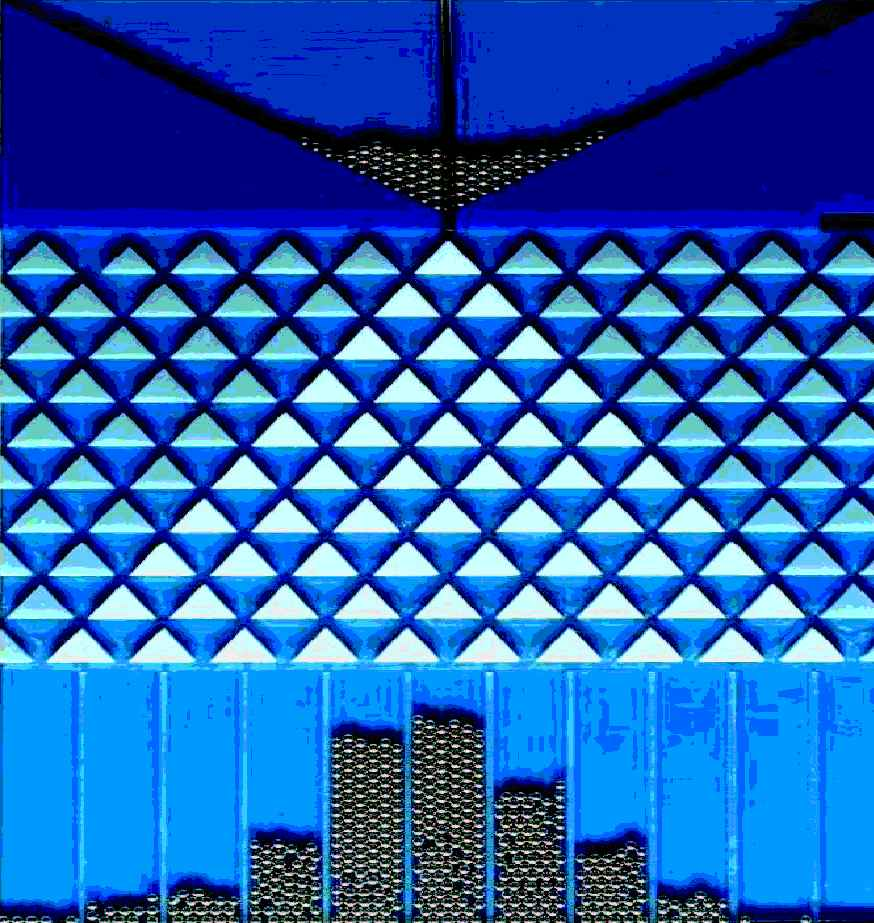
\includegraphics[width=0.9\columnwidth]{imagens/Normal.png}
  \caption{Modelo físico demonstrando a gênese da distribuição normal. FONTE: \cite{1}}
  \label{fig:normal}
\end{figure}
\vskip1ex

\vskip1ex
\begin{figure}
  \centering
  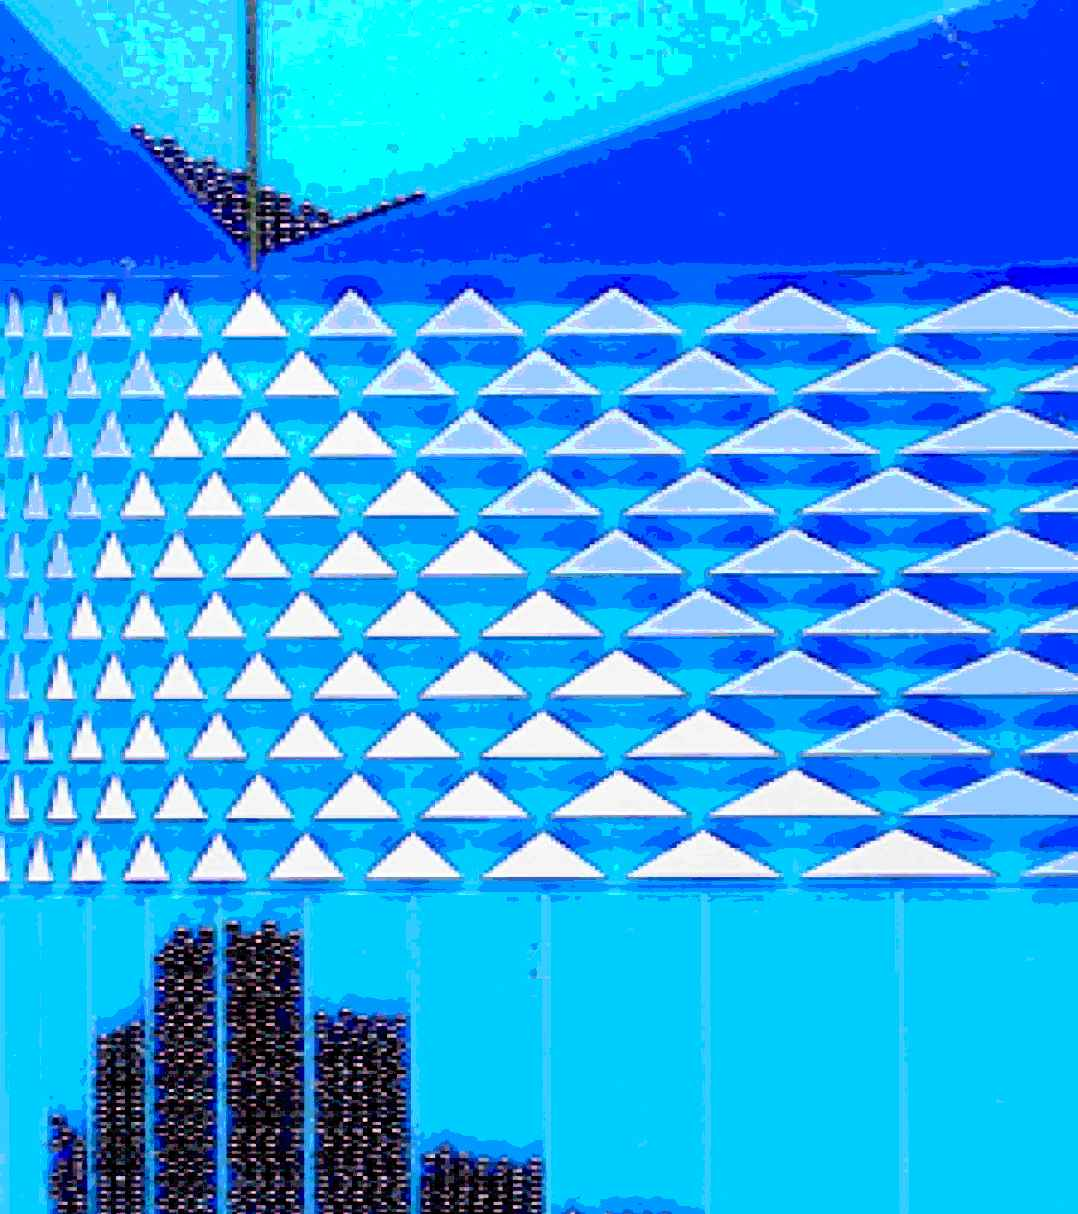
\includegraphics[width=0.9\columnwidth]{imagens/Lognormal.png}
  \caption{Modelo físico demonstrando a gênese da distribuição lognormal. FONTE: \cite{1}}
  \label{fig:lognormal}
\end{figure}

\vfill\null
\columnbreak

\section{Características}

\subsection{Medidas de tendência central}

Na distribuição lognormal, diferentemente do que ocorre nas distribuições simétricas,
como a distribuição normal, moda, média e mediana tem valores distintos,
o que pode ser observado na figura \ref{fig:normal_lognormal}.

\vskip1ex
\begin{figure}
  \centering
  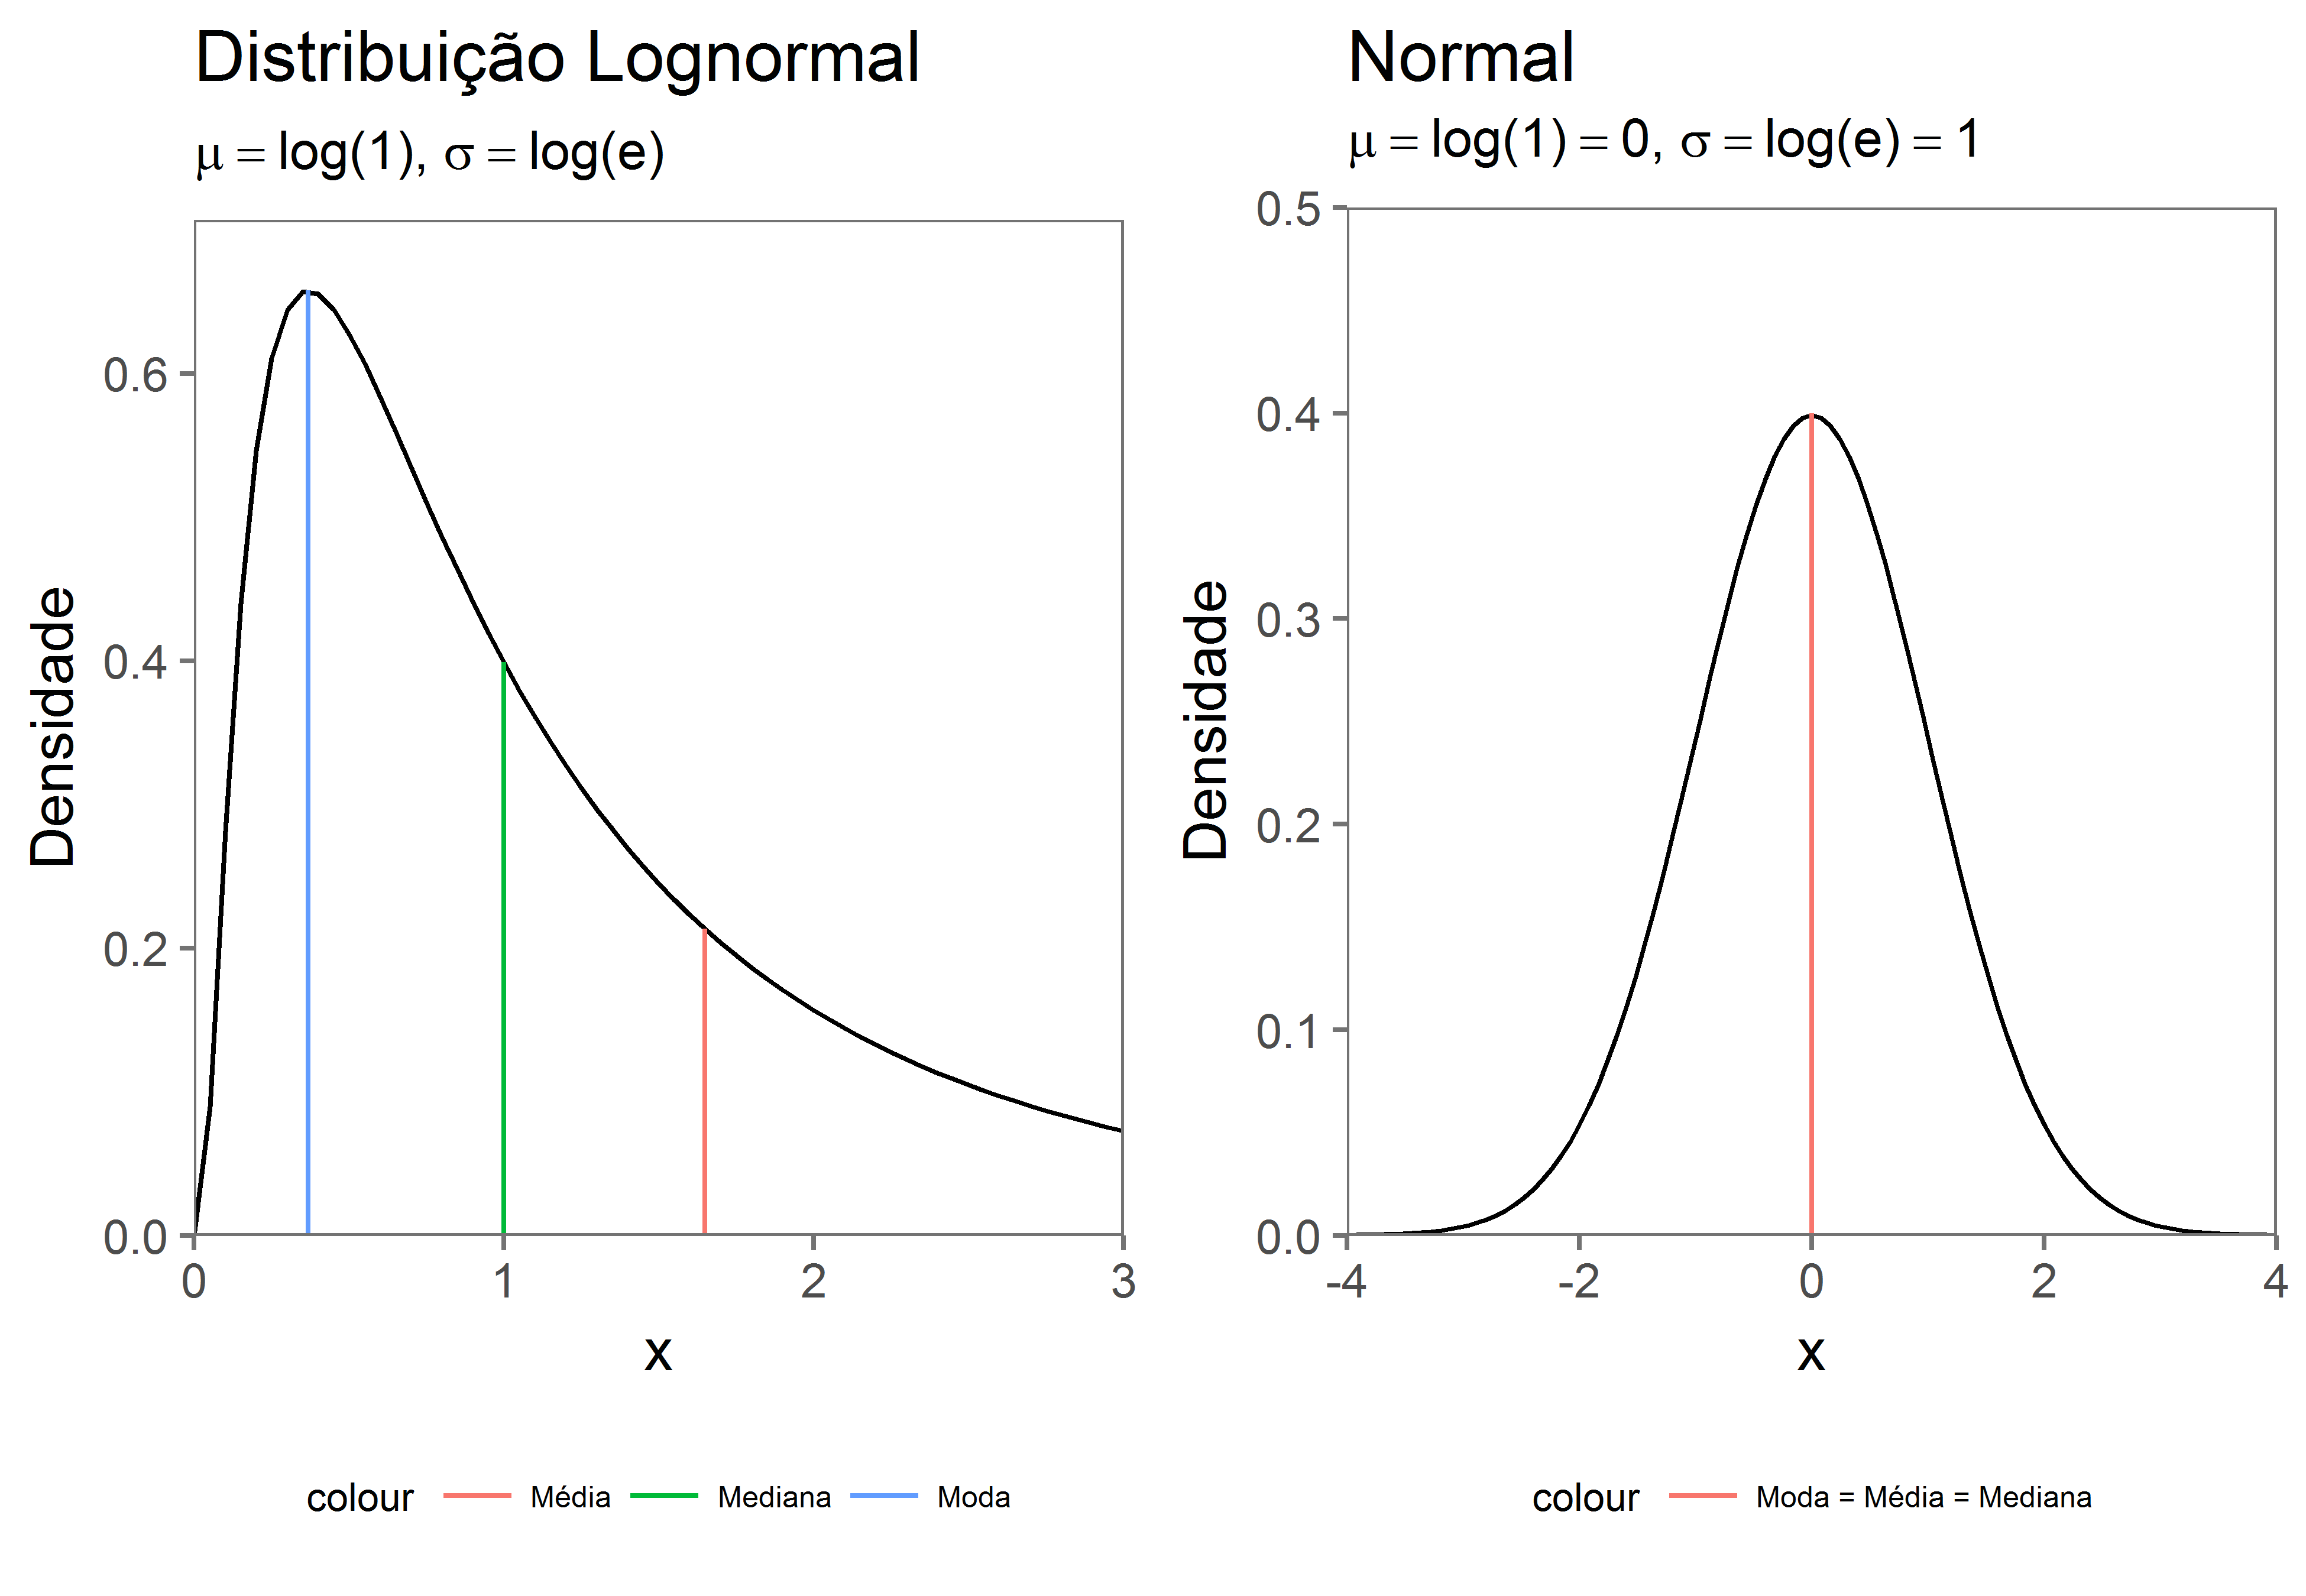
\includegraphics[width=0.99\columnwidth]{E:/Documents/Artigos/Dist_lognormal/images/normal_lognormal-1.png}
  \caption{Comparação entre distribuição normal e lognormal. FONTE: Autor}
  \label{fig:normal_lognormal}
\end{figure}

\subsection{Formulação}

a. Função densidade de probabilidade

$$\begin{cases}
f(x;\mu, \sigma) = \frac{1}{x\sigma\sqrt{2\pi}}\exp(-\frac{(log(x) - \mu)^2}{2\sigma^2}) & \forall x > 0 \\
0 & \text{ se } x = 0
\end{cases}$$

b. Valor Esperado (Média)

$$\mathbb{E}(X) = \exp \left ( \mu + \frac{\sigma^2}{2} \right )$$

c. Moda

$$Mo = \exp \left ( \mu - \sigma^2 \right )$$

d. Mediana

$$\nu = \exp \left ( \mu \right )$$

e. Variância

$$\newcommand{\Var}{\operatorname{Var}} \Var(X) = \exp (2\mu+\sigma^2)(\exp(\sigma^2)-1)$$

$$\newcommand{\Var}{\operatorname{Var}} \Var(X) = \mathbb{E}^2(X)(\exp(\sigma^2)-1)$$

f. Coeficiente de Variação

$$CV = \sqrt{\mathrm{e}^{\sigma^2}-1}$$

g. Parâmetros na escala anti-logarítmica

$$\mu^* = \mathrm{e}^\mu$$
$$\sigma^* = \mathrm{e}^\sigma$$

h. Intervalos de Confiança

\begin{description}
  \item[@68,3\% ($1\sigma$)]
  $$[\mu^*/\sigma^*; \mu^* \cdot \sigma^*]$$
  \item[@95,5\% ($2\sigma$)]
  $$[\mu^*/(\sigma^*)^2; \mu^* \cdot (\sigma^*)^2]$$
\end{description}


\vfill\null
\columnbreak

\subsection{Estimação dos parâmetros}

A melhor maneira de estimar os parâmetros de dados lognormais é através do cálculo
dos parâmetros na escala logarítmica.

Por exemplo, seja $X$ uma variável aleatória com distribuição aproximadamente 
lognormal.Para estimar o parâmetro $\mu(X)$, primeiro estima-se o valor da média 
da variável $\ln(X)$, $\bar{x}$, e depois retorna-se para a estimava do parâmetro $\mu$ 
na escala original através da transformação inversa ($\mu = \exp(\bar{x})$).

\section{Resultados}

No que tange à Engenharia de Avaliações, um dos aspectos mais importantes é o de qual
seria a melhor medida de tendência central a se adotar para estimar o valor do bem.

Na tabela 1 mostramos que a adoção da média, moda ou mediana é praticamente irrelevante
quando o erro-padrão $\sigma$ da regressão é pequeno. Porém, para altos valores de $\sigma$,
percebe-se uma discrepância muito grande entre os valores obtidos com a média, moda ou mediana.

Para efeito de comparação, a tabela 1 mostra os valores da moda e da média em função
do desvio-padrão $\sigma$, quando a mediana da distribuição tem valor fixado em
$\mu^* = 1.000.000$.

\vskip1ex
\begin{table}
  \rowcolors{2}{gray!25}{white}
  \centering
  \caption{Moda e Média em função do desvio-padrão, quando $\mu$ = 1.000.000. FONTE: Autor.}
  \begin{tabular}{ccccc}
    \rowcolor{gray!50}
    \hline\hline
    Medida / $\sigma$ & 0,1 & 0,25 & 1,0 & 2,0\\
    \hline
    Moda & 990.050 & 939.413 & 367.879 & 18.316\\
    \% & -1,0\% & -6,1\% & -63,2\%  & -98,2\%\\
    Média & 1.005.013 & 1.031.743 & 1.648.721 & 7.389.056\\
    \% & +0,5\% & +3,2\% & +64,9\% & +638,9\%\\
    IC @68,3\% & 904.837 & 778.800 & 367.879	& 135.335\\
    (1 $\sigma$) &  1.105.170 & 1.284.025 & 2.718.281 & 7.389.056 \\
    IC @95,5\% & 818.731 & 606.531 & 135.335 & 18.316\\
    (2 $\sigma$) & 1.221.403 & 1.648.721 & 7.389.056 & $54,6 x 10^6$\\
    \hline\hline
  \end{tabular}
\end{table}
\vskip2ex

Em suma, fixado $\mu^*$, à medida que o desvio-padrão aumenta, a moda da 
distribuição tende a zero, enquanto a média da distribuição tende a $+\infty$.

\section{Outros detalhes}

Para saber mais sobre a distribuição lognormal, visitar o \cite{site}.

%==============================================================================
%==End of content==============================================================
%==============================================================================

%--References------------------------------------------------------------------

\section{Referências}

\begin{thebibliography}{99}
  \bibitem{1} LIMPERT, E.; STAHEL, W.A.; ABBT, M. Log-normal Distributions across 
  the Sciences, \textit{BioScience}
  \bibitem{2} J.~Doe, J. Smith, Other article name, \textit{Phys. Rev. Lett.}
  \bibitem{site} \url{http://droubi.me/dist_lognormal/}
\end{thebibliography}

%--End of references-----------------------------------------------------------

\end{multicols}

%==============================================================================
\end{frame}
\end{document}
